%\clearpage
\section{Datenserver (AW)}
\label{section_datenserver}
Der Datenserver nimmt über eine Schnittstelle im REST-Design\footnote{REST 
(Representational State Transfer): Programmierparadigma, um Ressourcen im Web über 
definierte und eindeutige Schnittstellen zu erreichen} Anfragen über HTTP\footnote{HTTP 
(Hyper Text Transfer Prototcol)} entgegen und wandelt diese in Datenbankanfragen um. 
Nach erfolgter Antwort gibt der Datenserver die Daten aus der Datenbank an den Client 
über HTTP zurück.

Der Ablauf der beschriebenen Kommunikation ist in Abbildung 
\ref{fig_kommunikation_webserver_datenserver} ersichtlich:

\begin{figure}[h]
	\centering
	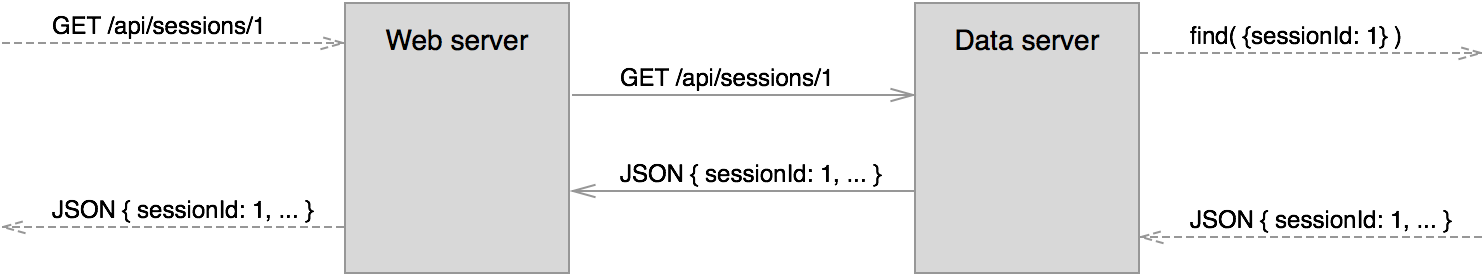
\includegraphics[width=\textwidth]{bilder/abbildung_request_from_webserver_to_dataserver}
	\caption{Kommunikation zwischen Webserver und Datenserver}
	\label{fig_kommunikation_webserver_datenserver}
\end{figure}

Die Abbildung zeigt, wie am Webserver eingehende Requests an den Datenserver weitergeleitet werden.
Der Datenserver erstellt daraufhin eine Datenbankanfrage und verarbeitet die erhaltene 
Antwort. Diese wird an den Webserver gesendet, der sie an den Webclient weiterleitet.

\subsection{Schnittstellen}
Die Endpunkte der Schnittstelle, die der Datenserver zur Kommunikation anbietet, 
sind der folgenden Tabelle \ref{tab_dataserver_api_routes} zu entnehmen:

\begin{table}[h]
	\begin{center}
		\begin{tabularx}{\textwidth}{|c|l|X|}
			\hline
			\textbf{Methode} & \textbf{Pfad} & \textbf{Funktion}\\
			\hline
			GET & /api/sessions/:id & ruft die Daten der Session mit der gegebenen ID auf \\
			\hline
			GET & /api/thumbnails/:id & ruft ein Thumbnail des Bildes mit gegebenen ID ab \\
			\hline
			GET & /api/images/:id & ruft ein Bild mit gegebenen ID ab \\
			\hline
		\end{tabularx}
		\caption{Die zu realisierende Schnittstelle}
		\label{tab_dataserver_api_routes}
	\end{center}
\end{table}

Die angegebenen Routen entsprechen denen des Webservers und dienen der Übermittlung 
der in der Datenbank hinterlegten Daten an den Webserver.

Der Datenserver hält noch weitere Schnittstellen bereit, um die Daten in die Datenbank einzutragen
und zu aktualisieren. Da das Einpflegen neuer Daten auch mit anderen Anwendungen und losgelöst
von der hier vorgestellten Anwendung erfolgen kann, wird hier des Umfangs wegen auf die Darstellung verzichtet.

\subsection{Realisierung}
Die Struktur der Anwendung wird in Abbildung \ref{fig_struktur_datenserver} ersichtlich:

\begin{figure}[h]
	\centering
	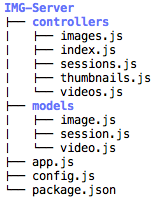
\includegraphics[width=4cm]{bilder/ordnerstruktur_datenserver}
	\caption{Ordnerstruktur Datenserver}
	\label{fig_struktur_datenserver}
\end{figure}

Der Aufbau des Datenserver entspricht größtenteils dem in Abschnitt \ref{section_webserver} beschriebenen Aufbau des Webservers.

Die Dateien \textit{app.js}, \textit{config.js} und \textit{package.json} erfüllen 
den gleichen Zweck wie auch beim Webserver.

Der Ordner \textit{controllers} enthält die Routen für die einzelnen Endpunkte der Schnittstelle.

Neu im Vergleich zum Webserver ist hier der Ordner \textit{models}, der Abstraktionen 
für den Zugriff auf die Datenbank bereithält. %\clearpage

Im folgenden Listing \ref{list_session_controller_model} ist beispielhaft die Reaktion 
auf eine Anfrage nach einer bestimmten Session dargestellt:

\begin{figure}[h]
	\begin{lstlisting}[caption={Auszug aus den Dateien controllers/sessions.js und models/session.js}, label=list_session_controller_model]
	(...)
	/*
	* GET request to /api/sessions/:id.
	* Returns the session with the requested id.
	*/
	router.get('/:id', function(req, res) {
		// get id from request parameters
	    var id = req.params.sessionId;
	    // use Session model to make db query
		Session.getOne(parseInt(id), function(result) {
			// if a result is found, send back the result
			if (result) {
				res.json(result);
			// otherwise send back a 404 status	
			} else {
				res.status(404).send();
			}
		});
	});
	
	(...)
	
	/*
	* Returns the session with the given id.
	* @param id - the id you're looking for
	* @param cb - a callback function
	* @returns a session object
	*/
	Session.getOne = function(id, cb) {
		mongoCrud.read({sessionId: id}, COLLECTIONNAME, function(doc) {
			cb(doc);
		});
	};
	\end{lstlisting}
\end{figure}

In den Zeilen 6 - 19 ist der Controller für den Pfad "/api/sessions/:id"{} zu sehen.
Dieser entnimmt den Request-Parametern die zu suchende ID und nutzt das Session-Model,
um eine Datenbankanfrage durchzuführen. Eine gefundene Session wird an den Client
(in diesem Fall der Webserver) zurückgegeben. Wird keine Session gefunden, wird der 
Statuscode 404 ("nicht gefunden") zurückgesendet.\clearpage

Die Zeilen 23 - 33 enthalten die Definition der Methode \textit{getOne} auf dem Modell \textit{Session}.
Darin wird mithilfe des Moduls \textit{mongo-crud-layer} (hier: mongoCrud) eine Suchanfrage
an die Datenbank gerichtet. Das Resultat dieser Abfrage, die Session-Daten oder ein Fehler, 
werden in übergebenen Callback-Methode verarbeitet.